\documentclass{standalone}
\usepackage{tikz}
\usepackage{ctex,siunitx}
\setCJKmainfont{Noto Serif CJK SC}
\usepackage{tkz-euclide}
\usepackage{amsmath}
\usetikzlibrary{patterns, calc}
\usetikzlibrary {decorations.pathmorphing, decorations.pathreplacing, decorations.shapes,}
\begin{document}
\small
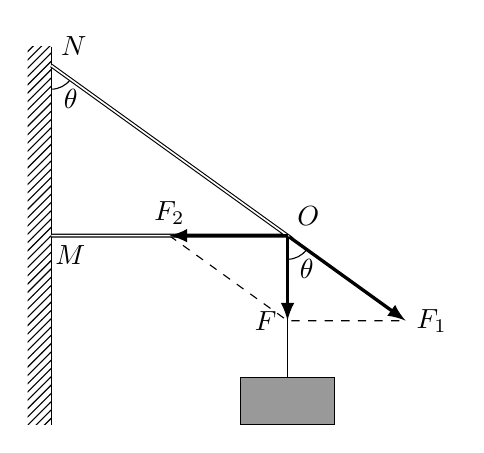
\begin{tikzpicture}[>=latex,scale=1.2]
  % \useasboundingbox(-1,-0.75)rectangle(3.7,1.4);
  \fill [pattern = north east lines] (-0.25,-2) rectangle (0,2);
  \draw (0,-2)--(0,2);
  \draw[->, very thick](2.5,0)--(2.5*1.5, -.9)node [right]{$F_1$};
  \draw[->, very thick](2.5,0)--(2.5,-.9)node [left]{$F$};
  \draw (2.5,0)--(2.5, -1.5);
  \draw[dashed](2.5*.5, 0)--(2.5,-.9)--(2.5*1.5, -.9);
  \draw[fill=black!40](2,-2) rectangle (3,-1.5);
  \draw (0,1.8-.25) arc(270:325:.25) node [below]{$\theta$};
  \draw (2.5,0-.25) arc(270:325:.25) node [below]{$\theta$};
  \draw[double] (0,1.8)node [above right]{$N$}--(2.5,0)node [above right]{$O$}--(0,0);
  \draw[very thick,->](2.5,0)--(2.5*.5, 0)node [above]{$F_2$};
  \node at (.2,-.2) {$M$};
  \end{tikzpicture}
\end{document}